\begin{prob}
Run Bellman-Ford on the following graph using node $s$ as the source.
Below each node $u$, write the shortest path length from $s$ to $u$.
    Mark the predecessor of $u$ by highlighting it or making a bold arrow.
    You can assume that \python{graph.edges} produces the graph's edges in the following
    order:
    \[(u_3, u_5), (u_1, u_2), (u_5, u_6), (u_4, u_8), (u_6, u_7), (s, u_1), (u_5, u_3),\] \[(u_1, u_8), (u_6, u_8), (u_8, u_4), (s, u_3), (u_2, u_4), (u_1, u_6), (u_8, u_2) \]
    
    $$
        \hspace{1em}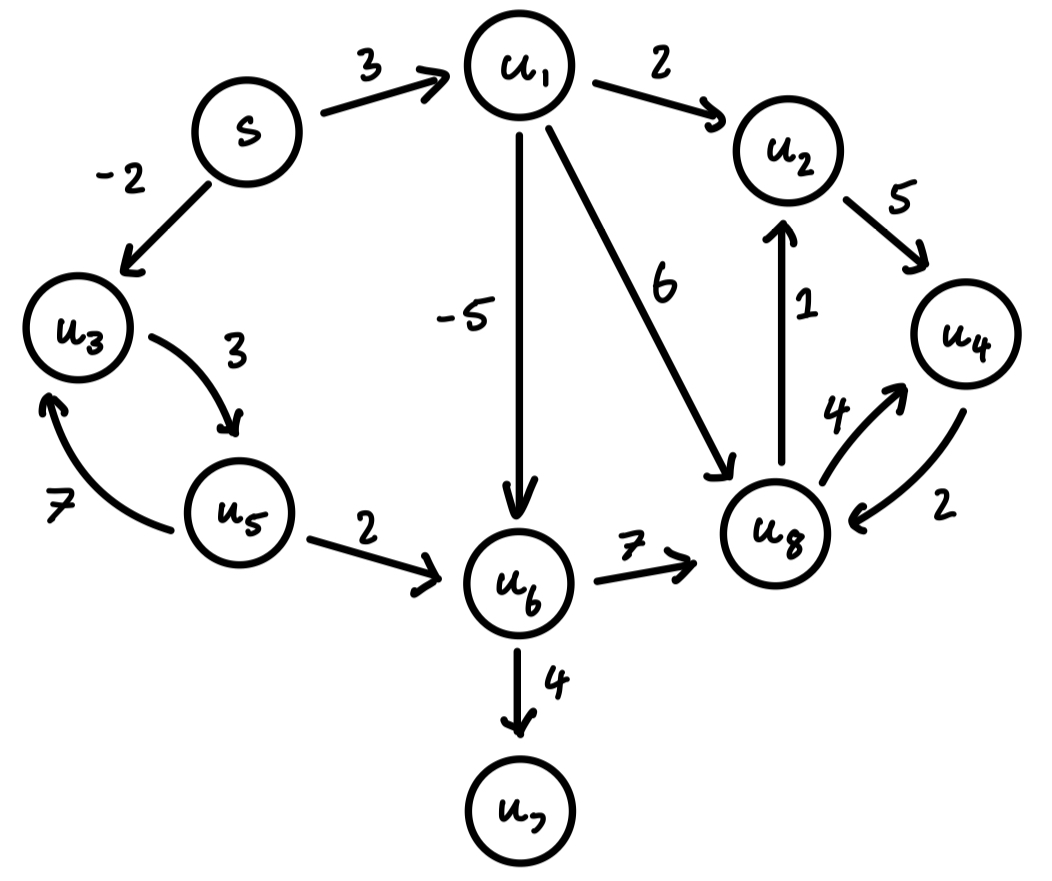
\includegraphics[scale = .24]{problems-hw-08/Q-1/HW8_1.jpeg}
    $$

    \begin{soln}
    %include your figure here
    
     
    \end{soln}
    
\end{prob}